\documentclass[10pt,a4paper,oneside]{scrartcl}

%\usepackage[ngerman]{babel}   % Deutsches Proposal
\usepackage[USenglish]{babel} % English proposal

\usepackage[utf8]{inputenc}
\usepackage{hyperref,xcolor,microtype,ifthen}

\setkomafont{disposition}{}
\setkomafont{descriptionlabel}{\bfseries}

\usepackage[textwidth=450pt]{geometry}

\usepackage[backend=bibtex,style=ieee,hyperref,natbib]{biblatex}

\usepackage{graphicx}
\graphicspath{{./res/}}

\usepackage{pgf-umlcd}

\addbibresource{references.bib}

% Kommentare abschalten
% Disable the hints here
\newboolean{showhints}
\setboolean{showhints}{true}
%\setboolean{showhints}{false}

\newcommand\hint[2]{
\ifthenelse{\boolean{showhints}}{
\begin{center}
\colorbox{black!10}{
\begin{minipage}{.963\textwidth}
#2\hfill\textbf{#1}
\end{minipage}
}\end{center}}{}
}

%Title of the proposal
\title{Automatic Change Recommendation using Decision Trees}
%bachelor or master?
\subtitle{Bachelor Thesis Proposal}
%first and then last name
\author{Valentin Reyes Häusler}

\begin{document}

\maketitle

\section{\iflanguage{ngerman}{Einführung und Motivation}{Introduction and Motivation}}
\label{sec:motivation}

- Design phase is a core step in any software development process
\\
- Objective of design phase: creation of design for architecture, software components, interfaces and data (IEEE-Standard "design phase")
\\
- This is accomplished by creating models and meta-models describing the solution precisely and completely while maintaining a necessary level of abstraction. (Skript 07.1)
\\
- For example: In object-oriented modeling class diagrams are indispensable. \ref{classDiag} shows classes and their relationships such as dependencies and associations. 
\\
- Importance of models: 
Recognition of patterns and redundancies allowing simplification (creation of a super class) 
... (TODO: more examples)
\\
- It is clear that a precise and complete design serves as a stable base for an efficient implementation.
\\
- Tools for the latter phase are vastly available. They range from code completion and action recommendation to generation of complete blocks of code.
\\
- This allows the engineer to concentrate on the core tasks of the implementation phase.
\\
- Although the design phase is equally important, comparable tools are often lacking or non existent.
\\
- A possible improvement in this aspect are automatic action proposals for the creation of models.
\\
- Basic to semi-complex actions such as the creation of a super class, separation of packages and so on, could be proposed to the designer.
\\
- Such a tool would again allow the engineer to concentrate on the core tasks of a consistent and complete design.
\\
- This thesis aims to create and evaluate such a tool.
\\
- We intend to do this by analyzing the versionized histories of models
\\
- Using machine learning algorithms and data structures we look for reoccurring patterns
\\
- The patterns are then matched to a model which is being worked on. 
\\
- If a fit is found a recommendation can be done.
\\
- Example for class diagrams:\\
Pattern:
State: Two classes X and Y share some attributes and functions\\
Actions: \\
\begin{itemize}
	\item Create superclass Z for X and Y
	\item Move shared attributes and functions from Y to Z
	\item Delete the same attributes and functions from X
\end{itemize}
Abstraction: Pull up shared attributes/functions to superclass
\begin{center}
	\begin{figure}
		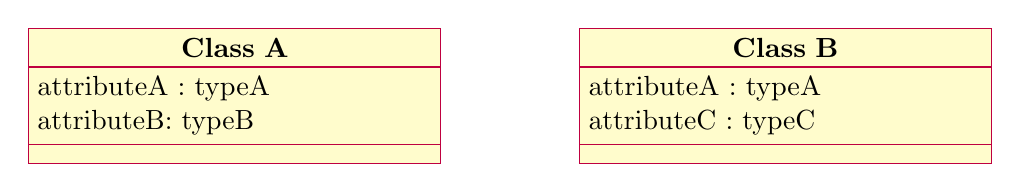
\begin{tikzpicture}
		\begin{class}{Class A}{0,0}
		\attribute{attributeA : typeA}
		\attribute{attributeB: typeB}
		\end{class}
		
		\begin{class}{Class B}{7,0}
		\attribute{attributeA : typeA}
		\attribute{attributeC : typeC}
		\end{class}
		\end{tikzpicture}
		\caption{Class diagram. Class A and class B share attributeA.}
	\end{figure}
\end{center}

\begin{center}
	\begin{figure}
		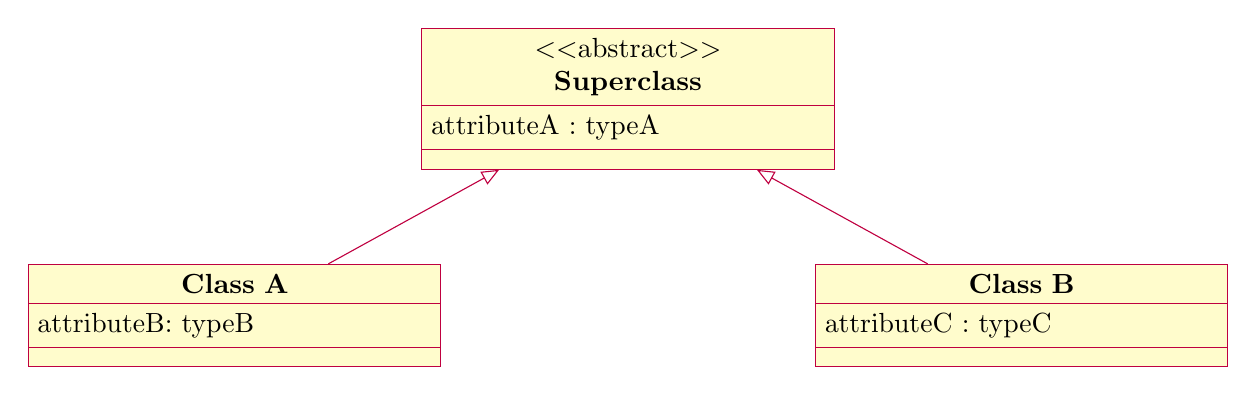
\begin{tikzpicture}
		\begin{abstractclass}{Superclass}{0,0}
		\attribute{attributeA : typeA}
		\end{abstractclass}
		
		\begin{class}{Class A}{-5,-3}
		\inherit{Superclass}
		\attribute{attributeB: typeB}
		\end{class}
		
		\begin{class}{Class B}{5,-3}
		\inherit{Superclass}
		\attribute{attributeC : typeC}
		\end{class}
		\end{tikzpicture}
		\caption{attributeA is "pulled up" from class A and B to Superclass. }
	\end{figure}
\end{center}
\section{\iflanguage{ngerman}
	{Problemstellung}
	{Problem Statement}}
\label{sec:problem_statement}

- We use SiLift
\\
- SiLift is able to compare different versions of a model
\\
- It recognizes \textit{low-level} actions and dependencies between those actions.
\\
- Low-level actions are simple internal operations for the deletion and creation of objects and their references.
\\
\begin{figure}
	\centering
	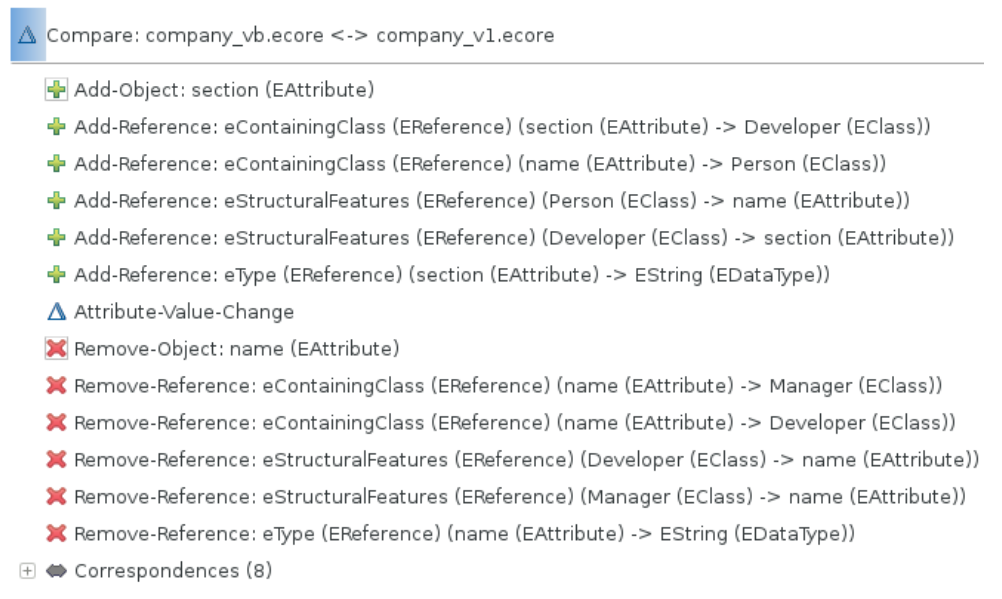
\includegraphics[width=0.9\textwidth]{./res/low-level-actions.png}
	\caption{Low-level differences between two models as recognized by SiLift}
	\label{fig:SiLiftEx}
\end{figure}
- Figure \ref{fig:SiLiftEx} shows the low-level differences between two versions of the model \textit{company}.
\\
- These low-level actions can be combined to \textit{user-level} actions. This can be seen in \ref{fig:SiLiftEx}.
\\
-Creating a new string-attribute \textit{section} in the class \textit{Developer} consists of:
\begin{enumerate}
	\item Create attribute: section
	\item Add containingClass-reference from section to Developer
	\item Add structuralFeatures-reference from Developer to section
	\item Add type-reference from section to String
	\item Change the value of section.
\end{enumerate}
- Abstracting the individual actions we can create a \textit{recognition rule} for the user-level action INSERT \textless type\textgreater \textless attr\textgreater=\textless val\textgreater IN \textless class\textgreater :
\begin{enumerate}
	\item Create attribute: \textless attr\textgreater
	\item Add containingClass-reference from \textless attr\textgreater to \textless class\textgreater
	\item Add structuralFeatures-reference from \textless class\textgreater to \textless attr\textgreater
	\item Add type-reference from \textless attr\textgreater to \textless type\textgreater
	\item Change value of \textless attr\textgreater to \textless val\textgreater
\end{enumerate}
- SiLift uses these recognition rules and \textit{lifts} matching sets of low-level actions to user-level actions.
\\

- We aim to automatically generate recognition rules from a models history.
\\
- The initial data is given in from of a dependency graph.
\\
\begin{figure}
	\centering
	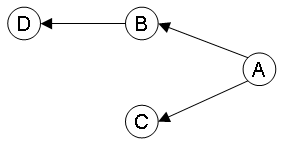
\includegraphics{./res/Dependencygraph.png}
	\caption{Dependency graph. A has to happen before B and C; B has to happen before D.}
	\label{fig:depgraph}
\end{figure}
- Nodes represent actions; edges dependencies.
\\
- Figure \ref{fig:depgraph} represents a dependency graph.
\\
- Note that since not every actions has a dependency there can be multiple nodes without parent nodes. And multiple node disjunct graphs.
\\
- We call this nodes orphan-nodes.
\\
- Generating the recognition rule for \textit{INSERT \textless type\textgreater \textless attr\textgreater=\textless val\textgreater IN \textless class\textgreater} we applied an abstraction to the low-level actions.
\\
-The abstraction consists of mapping the arguments of an action to variables.
\\
- For example: Create attribute: section becomes Create attribute: \textless attr0\textgreater with \textless attr0\textgreater = section.
\\
- Applying this abstraction allows us to compare actions and action sequences to one another.
\\
- We use this to find reoccurring patterns of action sequences in a model's history.
\\
- To do this we create multiple decision trees.
\\
- The generation of a decision tree is as follows:
\begin{enumerate}
	\item Find every orphan node representing the same abstract action.
	\item Create a decision tree with that action as it's root.
	\item For every orphan node do:
	\begin{enumerate}
		\item Breadth first search every possible path starting at the orphan node.
		\item If there is no equivalent path in the decision tree starting at the root, find the largest matching path starting at the root and expand it to match.
	\end{enumerate}
\end{enumerate}
- The construction of the decision trees allows us to calculate the frequency and with that the probability of a certain path happening.
\\
- With this data structure we can match the last actions of a user to the corresponding decision (sub-)tree and giving subsequent paths as possible actions.
\\
\\
- It is easy to see that this format could be expanded to be used in other applications where access to a versionied history is available.


\section{Purpose of the study}
The purpose of this study is to create a tool for change proposal during the creation of models and meta models. Such a tool, if efficient, could provide support for engineers during the design phase of software comparable to autocompletion tools used during the implementation phase. 

\section{\iflanguage{ngerman}
	{Verwandte Forschung}
	{Review of the literature}}

\iflanguage{ngerman}
{}
Until now only the comparable paper on automatic change recommendation has be studied. Further reading can be done for autocompletion algorithms for other applications. Decision trees, random forests and other regression data structures should be contemplated as well.


\section{\iflanguage{ngerman}
	{Forschungsfragen}
	{Research questions and/or Hypotheses}}
\label{sub:questions}

\iflanguage{ngerman}
{}
%
\begin{description}
\item[RQ1:] What are the problems when implementing change recommendation tools?
\item[RQ2:] How helpful is such a tool realistically?
\item[RQ3:] How well does the tool perform?
\item[RQ5:] How much data does the tool need to perform relatively well?
\item[RQ4:] How does the tool compare to other implementations?
\end{description}

\section{\iflanguage{ngerman}
	{Eigener Ansatz}
	{The Design - Methods and Procedures}}
\label{sec:approach}

\iflanguage{ngerman}
{}


\section{\iflanguage{ngerman}{Einschränkungen}{Limitations and Delimitations}}
The goal of this study is to create an effective and helpful change recommendation tool to aid during the creation of models. We will still aim to keep the tool as broad as possible so that it can be used for other application in which a change history is available.

Although a user interface and plugin for different model creation software are certainly imaginable, we won't try to archive those goals. Instead a command line interface will be implemented.


\section{\iflanguage{ngerman}{Signifikanz der Untersuchung}{Significance of the study}}
The significance of this study lies within its usability and helpfulness. Streamlining the process of model creation aids to increase the quality of software and its design. The ability to bypass mindless repetition during the creation of a model helps the engineer to focus on the important aspects of that model. 

The creation of this study will also help in deepening my knowledge in functional programming and machine learning. Both of which serve as useful tools for any programmer. With the former being an additional paradigm with which to program and the latter being a relevant topic in almost every aspect of computer science.


\section{\iflanguage{ngerman}
	{Planung}
	{Planning}}
\label{sec:planning}

\subsection{\iflanguage{ngerman}
	{Eigene Vorkenntnisse}
	{Own Background}}
\label{sub:background}
My knowledge in functional programming, while lean, serves as a good start for the creation of this study. Especially when supported by my background with lectures such as "Programmierung von Systemen" and "Algorithmen und Datenstrukturen" as a student as well as a tutor. Both of which are highly applicable in this study. My participation in "Sopra 16/17" provides me with experience for the designing, implementation and testing of the tool which we aim to create. 

Having said that, extensive practice in practical functional programming will be necessary as well as attaining knowledge in machine learning, especially regression algorithms. My successful completion of the lecture "Einführung in die künstliche Intelligenz" and the proseminar "Algorithmen" will hopefully provide a strong base for that.

\subsection{\iflanguage{ngerman}
	{Benötigte Ressourcen}
	{Required Resources}}
\label{sub:resources}
No especial resources will be necessary. Only access to data in form of model histories and the tool SiLift should suffice for the creation of this study.

\subsection{\iflanguage{ngerman}
	{Zeitplanung}
	{Work packages}}
\label{sub:wp}

\iflanguage{ngerman}

\begin{description}
\item[M1] Extensive research into regression learning and practice with practical Haskell.
\item[M2] Design and planning of the tool.
\item[M3] Implementation and testing.
\item[M4] Implementation and testing.
\item[M5] Review and possible correction of the tool.
\item[M6] Collection of results on paper, answering all research questions, including the comparison with comparable tools.
\end{description}

\subsection{\iflanguage{ngerman}
	{Risiken und Ausweichplan}
	{Contingency plan}}
\label{sub:contingency}

\iflanguage{ngerman}

\begin{enumerate}
\item Failing to create such a tool with Haskell due to lacking knowledge. This eventuality will be discussed with the creators of the study.
\end{enumerate}

\nocite{*}
\printbibliography

\end{document}

